\documentclass{beamer}
\usepackage[normalem]{ulem}
\usepackage[absolute,overlay]{textpos}
%\usetheme{Singapore}

\usepackage{pgfplots}
\pgfplotsset{compat=1.18}

%\include{preamble}

\usepackage{svg}

   
%\usecolortheme[RGB={204,51,255}]{structure}
%\usecolortheme[named=purple]{structure}
\usecolortheme[RGB={62,128,62}]{structure}
%\definecolor{dark}{rgb}{0.3,0.15,0.3}
%\definecolor{light}{rgb}{0.8,0.6,0.8}
\definecolor{reddish}{rgb}{.5,0.15,0.15}
\definecolor{rr}{rgb}{.5,0.15,0.15}
\definecolor{dark}{rgb}{0.4,0.2,0.4}
\definecolor{darkgreen}{rgb}{0.25,0.5,0.25}
\definecolor{darkred}{rgb}{0.75,0.25,0.25}
\definecolor{darkblue}{rgb}{0.25,0.25,0.75}
\definecolor{light}{rgb}{0.8,0.6,0.8}
\definecolor{reddish}{rgb}{.7,0.25,0.25}


\newcommand{\cored}{\color{red}{}}
\newcommand{\coblu}{\color{blue}{}}
\newcommand{\coblue}{\color{blue}{}}
\newcommand{\cor}{\color{reddish}{}}
\newcommand{\cob}{\color{black}{}}

\newcommand{\mm}[1]{\color{reddish}{}$#1$\color{black}{}}

\renewcommand{\S}[0]{\mathcal{S}}
\newcommand{\M}[0]{\mathcal{M}}
\newcommand{\B}[0]{\mathcal{B}}
\renewcommand{\P}[0]{\mathcal{P}}
\newcommand{\A}[0]{\mathcal{A}}
\newcommand{\egood}[0]{XCS\xspace}%e added to remind us to use "an" before
\newcommand{\oilm}[0]{Obverter ILM\xspace}
\newcommand{\ailm}[0]{Semi-Supervised ILM\xspace}

\newcommand{\BB}[0]{\mathbb{B}}
\renewcommand{\AA}[0]{\mathbb{A}}


\usepackage{graphicx}
\usepackage{pstricks}

\setbeamertemplate{navigation symbols}{}

\usepackage{tikz}
\usetikzlibrary{arrows,decorations.markings,positioning}
\usepackage{tikz-qtree}
\usepackage{epstopdf}

\newcommand{\signals}[0]{\color{blue}signals\color{black}{}}
\newcommand{\meanings}[0]{\color{red}meanings\color{black}{}}

\newcommand*\eiadfamily{\fontencoding{OT1}\fontfamily{eiad}\selectfont}
\usepackage[OT1]{fontenc}

\newcommand{\ile}[1]{\color{reddish}$$#1$$\color{black}{}}


\title[Latent spaces and autoencoders]{Latent spaces and autoencoders}
\author{\textbf{S}EMTM0051}
\institute{SEMT, U Bristol / \texttt{semtm0051.github.io}}
\date{2026-11}

\begin{document}

\maketitle


\begin{frame}
  \frametitle{Motivation}
\vskip 0.25cm
\textbf{T}oday we will look at \textsl{auto-encoders}; auto-encoders are sometimes useful in and of themselves, however we are studying them as part of our effort to understand what makes networks work and because they provide a language or description of what networks are doing.
\end{frame}

% in the preamble:
% \usepackage{tikz}
% \usetikzlibrary{decorations.pathreplacing}

\begin{frame}
  \frametitle{Auto-encoder}
\vskip 0.25cm
\begin{center}
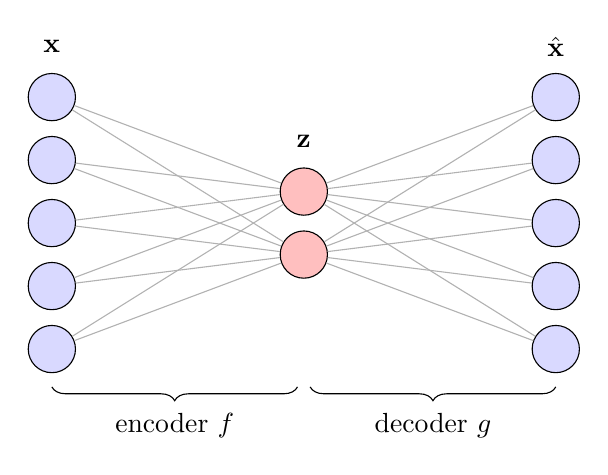
\begin{tikzpicture}[
    neuron/.style={circle,draw,minimum size=6mm,inner sep=0pt},
    edge/.style={gray!60},
    x=1.6cm,y=0.8cm]

  % input layer
  \foreach \i in {1,...,5}
    \node[neuron,fill=blue!15] (x\i) at (0,3-\i) {};

  % bottleneck
  \foreach \i in {1,2}
    \node[neuron,fill=red!25] (z\i) at (2,1.5-\i) {};

  % output layer
  \foreach \i in {1,...,5}
    \node[neuron,fill=blue!15] (y\i) at (4,3-\i) {};

  % connections
  \foreach \i in {1,...,5}
    \foreach \j in {1,2} {
      \draw[edge] (x\i) -- (z\j);
      \draw[edge] (z\j) -- (y\i);
    }

  % labels
  \node at (0,2.8)  {$\mathbf{x}$};
  \node at (2,1.3)  {$\mathbf{z}$};
  \node at (4,2.8)  {$\hat{\mathbf{x}}$};

  % encoder / decoder braces
  \draw[decorate,decoration={brace,mirror,amplitude=5pt}]
    (0,-2.6) -- (1.95,-2.6) node[midway,below=6pt] {encoder $f$};
  \draw[decorate,decoration={brace,mirror,amplitude=5pt}]
    (2.05,-2.6) -- (4,-2.6) node[midway,below=6pt] {decoder $g$};
\end{tikzpicture}
\end{center}
\vskip 0.2cm
\textbf{T}rain so that $\hat{\mathbf{x}}=g(f(\mathbf{x}))\approx\mathbf{x}$, for example by minimising $\|\mathbf{x}-\hat{\mathbf{x}}\|^2$.
\end{frame}

\begin{frame}
  \frametitle{Latent space}
\vskip 0.25cm
\begin{center}
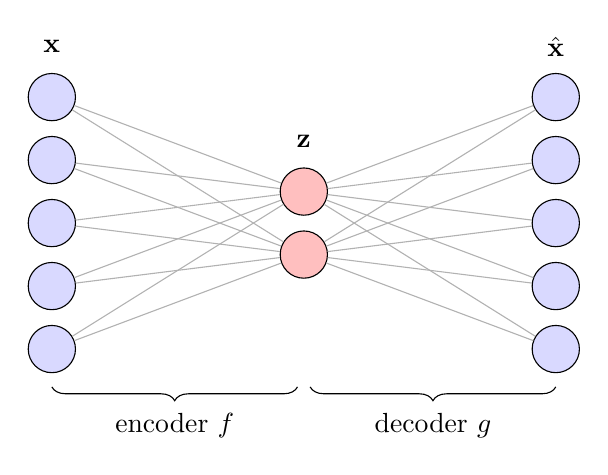
\begin{tikzpicture}[
    neuron/.style={circle,draw,minimum size=6mm,inner sep=0pt},
    edge/.style={gray!60},
    x=1.6cm,y=0.8cm]

  % input layer
  \foreach \i in {1,...,5}
    \node[neuron,fill=blue!15] (x\i) at (0,3-\i) {};

  % bottleneck
  \foreach \i in {1,2}
    \node[neuron,fill=red!25] (z\i) at (2,1.5-\i) {};

  % output layer
  \foreach \i in {1,...,5}
    \node[neuron,fill=blue!15] (y\i) at (4,3-\i) {};

  % connections
  \foreach \i in {1,...,5}
    \foreach \j in {1,2} {
      \draw[edge] (x\i) -- (z\j);
      \draw[edge] (z\j) -- (y\i);
    }

  % labels
  \node at (0,2.8)  {$\mathbf{x}$};
  \node at (2,1.3)  {$\mathbf{z}$};
  \node at (4,2.8)  {$\hat{\mathbf{x}}$};

  % encoder / decoder braces
  \draw[decorate,decoration={brace,mirror,amplitude=5pt}]
    (0,-2.6) -- (1.95,-2.6) node[midway,below=6pt] {encoder $f$};
  \draw[decorate,decoration={brace,mirror,amplitude=5pt}]
    (2.05,-2.6) -- (4,-2.6) node[midway,below=6pt] {decoder $g$};
\end{tikzpicture}
\end{center}
\vskip 0.2cm
\textbf{T}he space in the middle is called the \textsl{latent space}.
\end{frame}

\begin{frame}
  \frametitle{Motivation}
\vskip 0.25cm
$$\text{original}\rightarrow \text{latent representation} \rightarrow \text{reconstruction}$$
\textbf{T}he latent space should `pick out' what's important about the original so that it can reconstruct it even if the latent representation lives in a lower dimension! 
\end{frame}

\begin{frame}
  \frametitle{MNIST: origin}
\vskip 0.25cm
In the late 1980s LeCun and colleagues at Bell Labs were building networks to read ZIP codes on US mail.
\vskip 0.25cm
MNIST (1998) was built from two older NIST databases of handwritten digits:
\begin{itemize}
\item one written by US Census Bureau employees,
\item one written by high-school students.
\end{itemize}
\vskip 0.25cm
NIST had used the first for training and the second for testing, but the students' writing was harder to read, so MNIST mixes the two in both training and test sets: the ``M'' is for ``modified''.
\end{frame}

\begin{frame}
  \frametitle{MNIST: the data}
\vskip 0.25cm
\begin{itemize}
\item 60\,000 training images and 10\,000 test images.
\item Each is $28\times 28$ greyscale, a vector in $\mathbb{R}^{784}$.
\item Each has a label $0,\ldots,9$.
\end{itemize}
\vskip 0.25cm
\begin{center}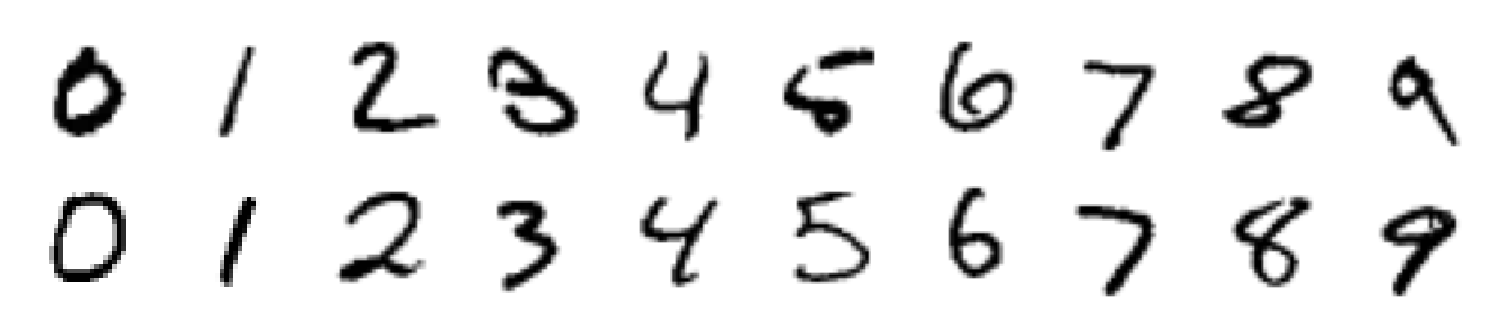
\includegraphics[width=0.8\textwidth]{mnist_samples.pdf}\end{center}
It is the standard beginner data set, and it is useful because the structure is simple: ten discrete categories plus noise, the noise being the variability of human handwriting.
\end{frame}

\begin{frame}
  \frametitle{MNIST: a caution}
\vskip 0.25cm
\textbf{I}t is too easy.
\begin{itemize}
\item Linear classifier: about $92\%$.
\item Small multilayer perceptron: about $98\%$.
\item Good convolutional network: about $99.7\%$.
\end{itemize}
\vskip 0.25cm
The last few errors are mostly ambiguous or mislabelled digits, so comparing good networks on MNIST probes the idiosyncrasies of the labelling, not the networks.
\vskip 0.25cm
For us that is fine: we want to see what a network is doing, not to win.
\end{frame}

\begin{frame}
  \frametitle{An autoencoder for MNIST}
\vfill
$$
784 \rightarrow 512 \rightarrow 256 \rightarrow 2 \rightarrow 256 \rightarrow 512 \rightarrow 784
$$
\vfill
\end{frame}

\begin{frame}
  \frametitle{An autoencoder for MNIST}
\vfill
$$
784 \rightarrow 512 \rightarrow 256 \rightarrow 2 \rightarrow 256 \rightarrow 512 \rightarrow 784
$$
\vskip 0.5cm
\begin{itemize}
\item Hidden layers: ReLU, $\phi(u)=\max(0,u)$.
\item Bottleneck: linear, so $\mathbf{z}\in\mathbb{R}^2$.
\item Output: sigmoid, so $\hat{x}_i\in[0,1]$.
\item Loss: binary cross-entropy,
$$
L=-\sum_{i=1}^{784}\left[x_i\log\hat{x}_i+(1-x_i)\log(1-\hat{x}_i)\right].
$$
\end{itemize}
\vfill
\end{frame}

\begin{frame}
  \frametitle{Reconstructions}
\vfill
\begin{center}
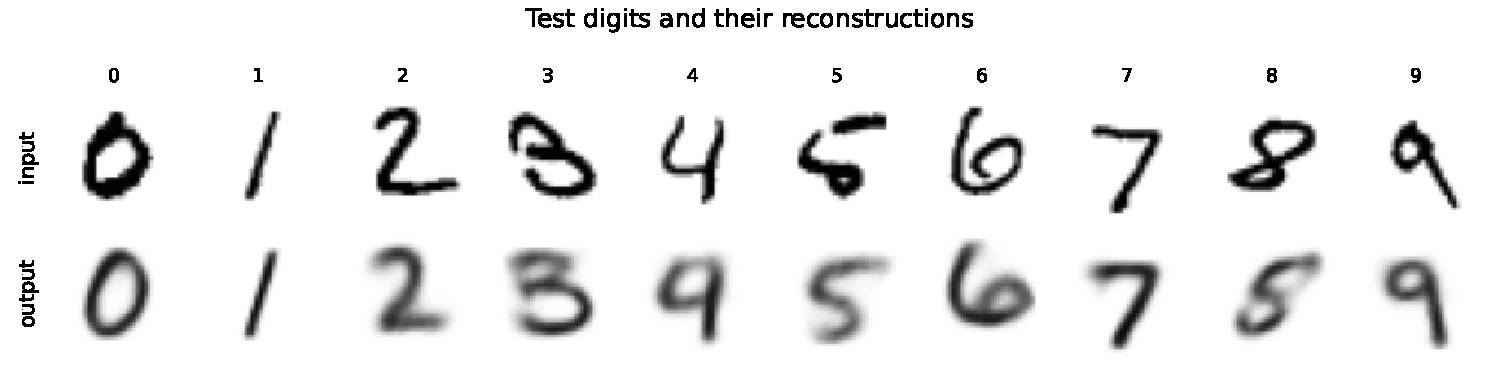
\includegraphics[width=\textwidth,height=0.7\textheight,keepaspectratio]{reconstructions.pdf}
\end{center}
\vfill
\textbf{E}ach digit is squeezed through two numbers and expanded back out again; the reconstructions are blurred but recognisable.
\end{frame}

\begin{frame}
  \frametitle{The worst reconstructions}
\vfill
\begin{center}
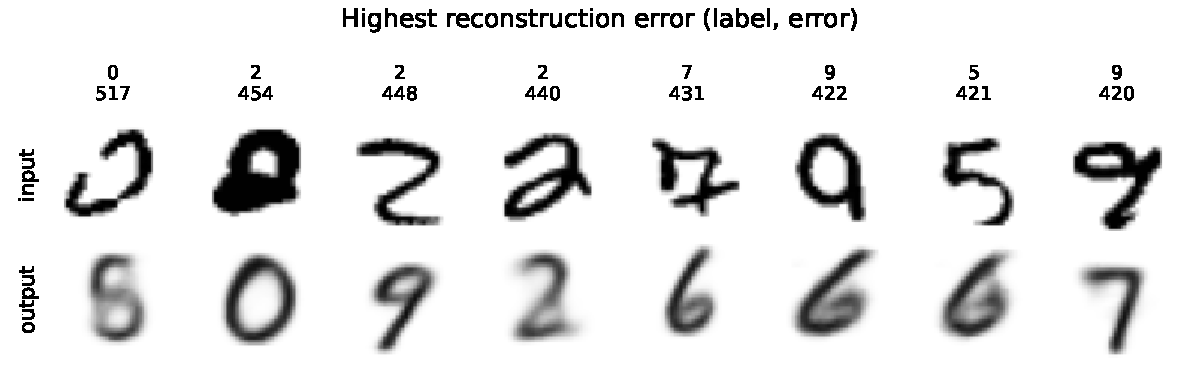
\includegraphics[width=\textwidth,height=0.7\textheight,keepaspectratio]{worst_reconstructions.pdf}
\end{center}
\vfill
\textbf{T}he test digits with the highest reconstruction error: mostly unusual or badly written digits, which the decoder replaces with something more typical.
\end{frame}

\begin{frame}
  \frametitle{The latent space}
\begin{center}
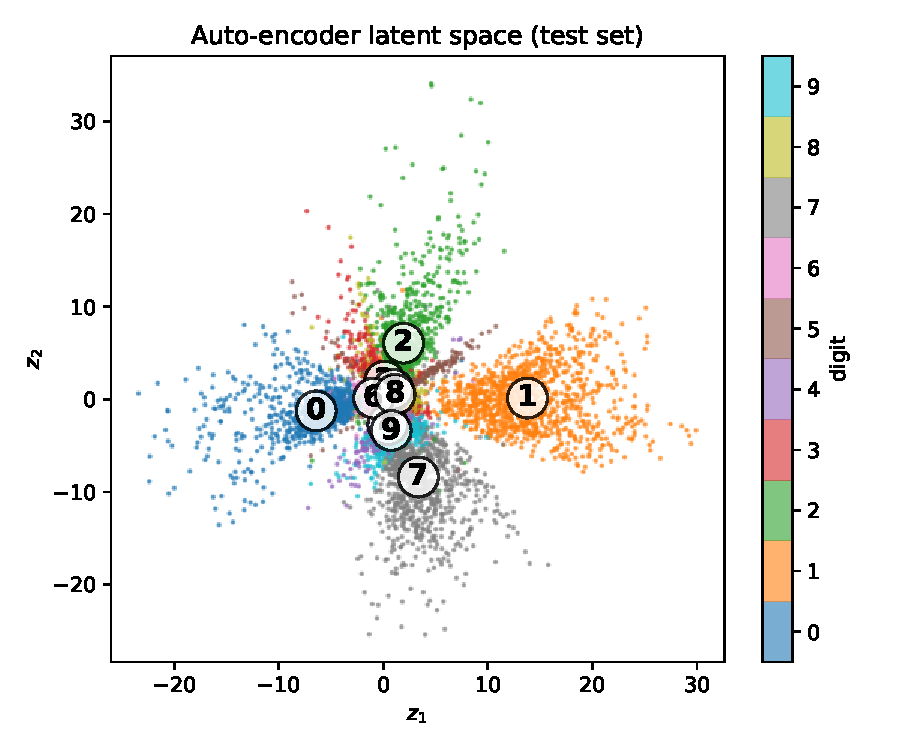
\includegraphics[width=\textwidth,height=0.82\textheight,keepaspectratio]{latent_scatter.pdf}
\end{center}
\end{frame}

\begin{frame}
  \frametitle{The latent space, zoomed in}
\begin{center}
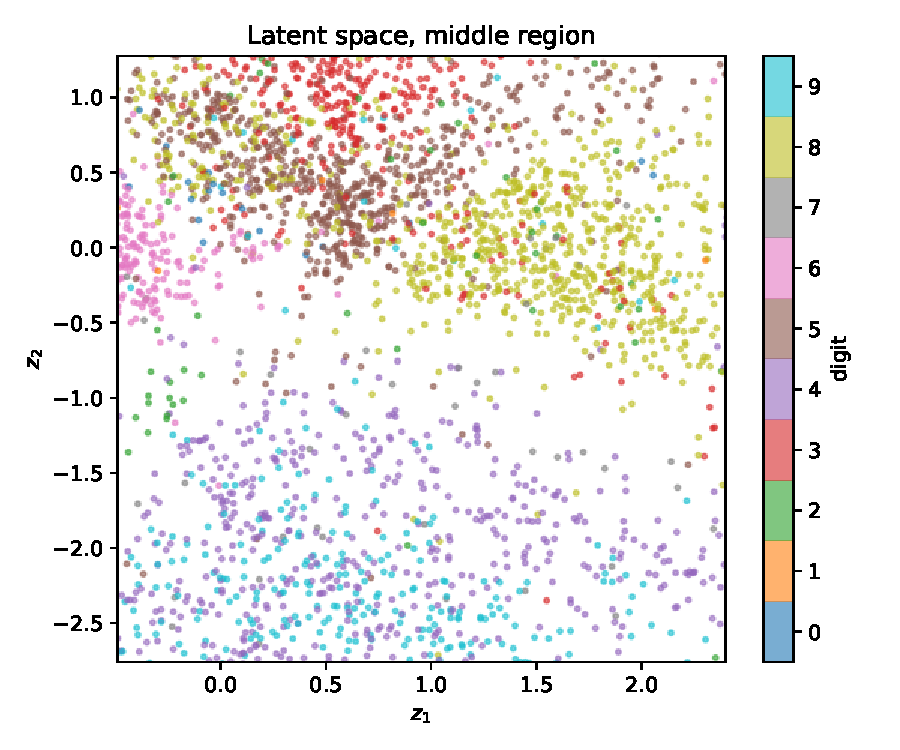
\includegraphics[width=\textwidth,height=0.82\textheight,keepaspectratio]{latent_scatter_zoom.pdf}
\end{center}
\end{frame}

\begin{frame}
  \frametitle{A line through latent space: 4 to 7}
\begin{center}
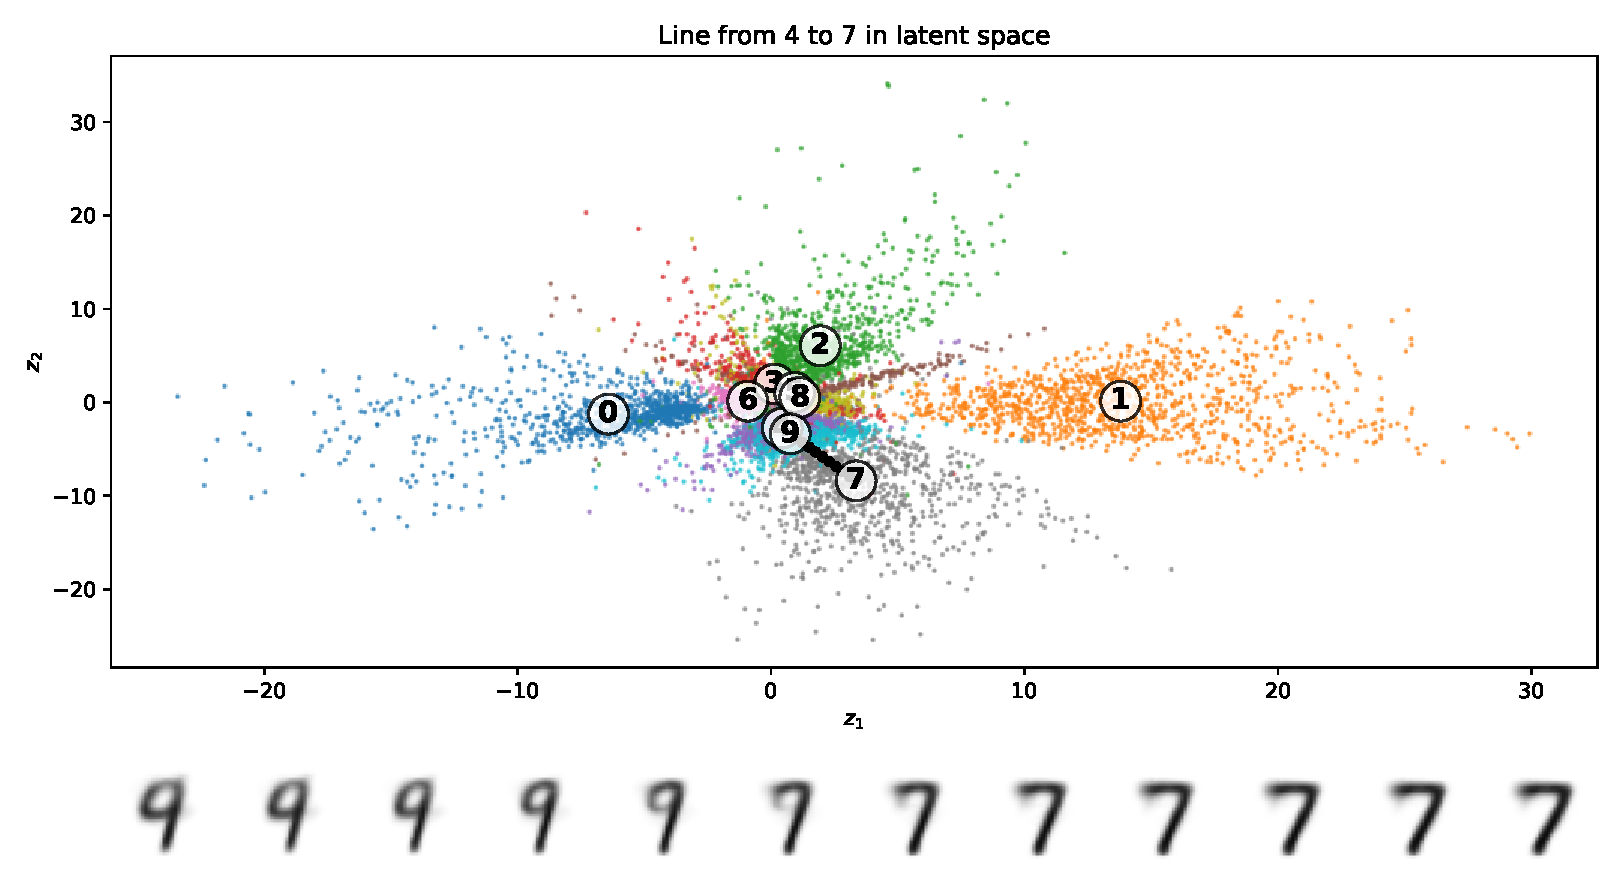
\includegraphics[width=\textwidth,height=0.72\textheight,keepaspectratio]{latent_line_4_7.pdf}
\end{center}
\textbf{T}he 4 cluster lies underneath the 9 cluster, so the line starts by decoding 9s: in two dimensions the decoder cannot tell them apart and gives the more typical digit.
\end{frame}

\begin{frame}
  \frametitle{A line through latent space: 1 to 0}
\begin{center}
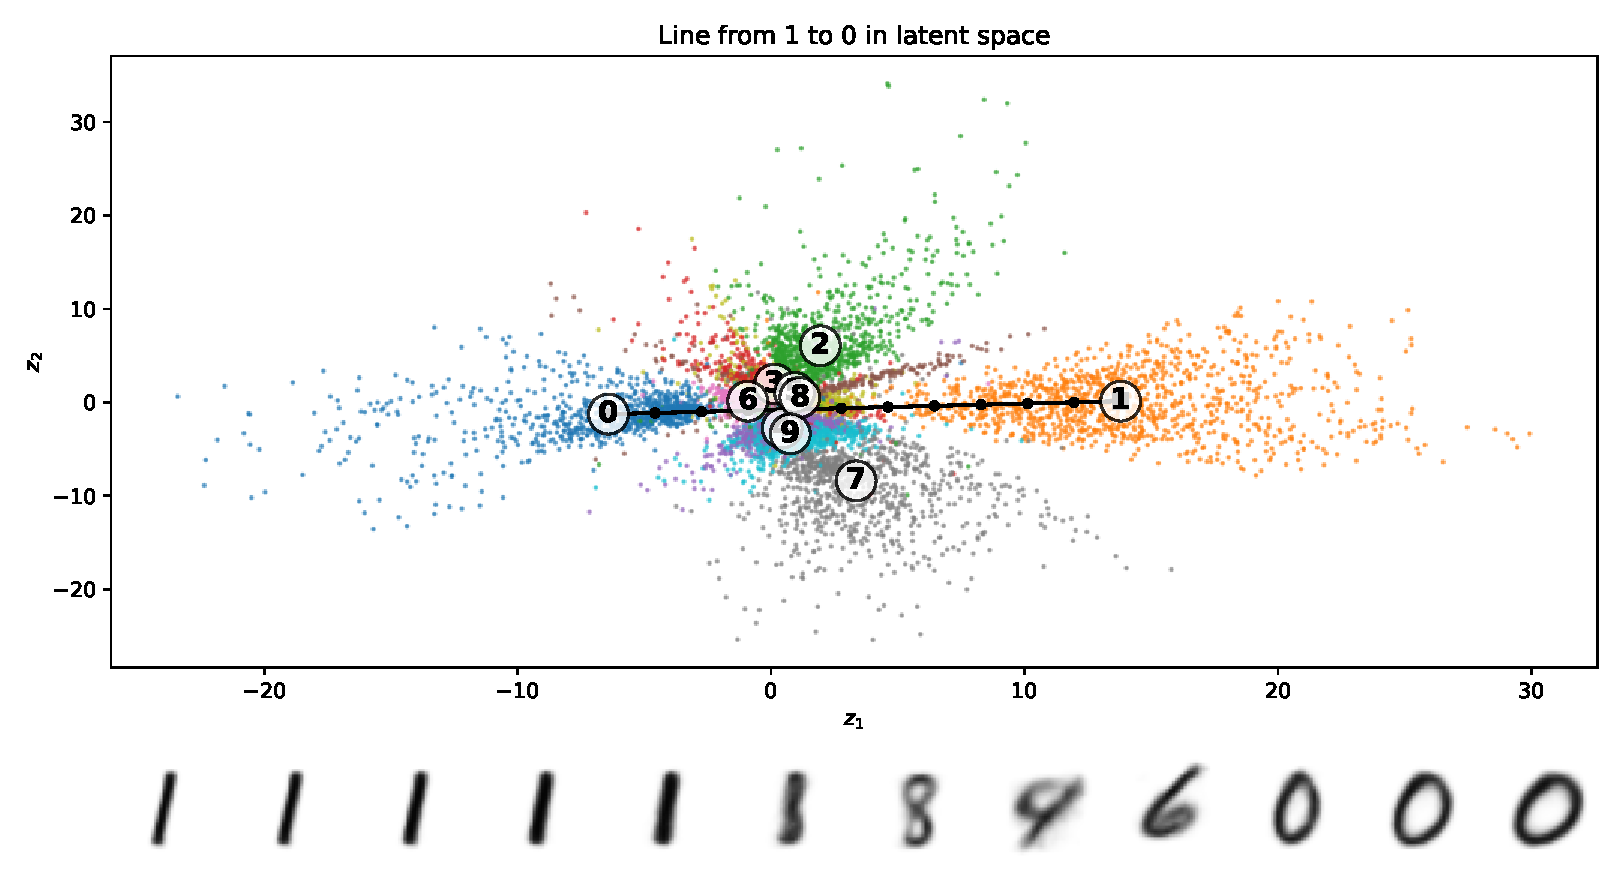
\includegraphics[width=\textwidth,height=0.72\textheight,keepaspectratio]{latent_line_1_0.pdf}
\end{center}
\textbf{A} straight line in latent space is not a straight path between digits: crossing the crowded middle we pass through 8, 4 or 9, and 6 on the way.
\end{frame}

\begin{frame}
  \frametitle{A circle in latent space}
\begin{center}
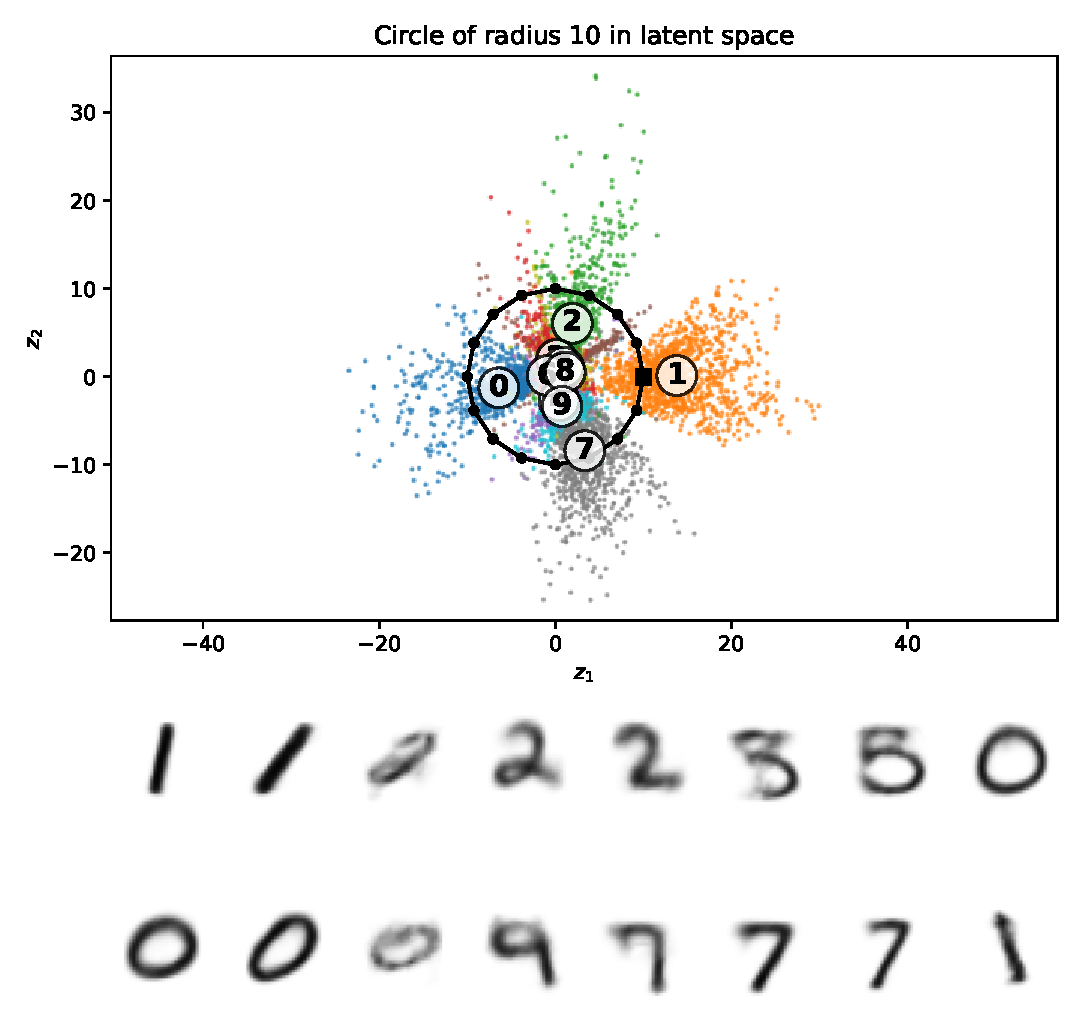
\includegraphics[width=\textwidth,height=0.82\textheight,keepaspectratio]{latent_circle.pdf}
\end{center}
\end{frame}



\begin{frame}
  \frametitle{Relationship with PCA}
\vfill
\textbf{Auto-encoder:}
$$
\text{original} \rightarrow \textcolor{red}{\text{latent}} \rightarrow \text{reconstruction}
$$
$$
\mathbf{x} \rightarrow \textcolor{red}{\mathbf{z}=f(\mathbf{x})} \rightarrow \hat{\mathbf{x}}=g(\mathbf{z})
$$
\vskip 0.5cm
\textbf{PCA:}
$$
\text{original} \rightarrow \text{PCA basis} \rightarrow \textcolor{red}{\text{top PCs}}
$$
$$
\mathbf{x} \rightarrow U^T\mathbf{x} \rightarrow \textcolor{red}{(\mathbf{u}_1^T\mathbf{x},\ldots,\mathbf{u}_k^T\mathbf{x})}
$$
\vfill
In both cases the data are summarised by $k$ numbers; for a \emph{linear} auto-encoder these turn out to be the same summary.
\vfill
\end{frame}

\begin{frame}
  \frametitle{The linear auto-encoder}
\vskip 0.25cm
\textbf{T}ake centred data $\mathbf{x}\in\mathbb{R}^n$ with covariance
$$
C=\frac{1}{N}\sum_a \mathbf{x}_a\mathbf{x}_a^T=U\Lambda U^T,\qquad \lambda_1\ge\lambda_2\ge\cdots\ge\lambda_n.
$$
\textbf{A} linear auto-encoder has $\mathbf{z}=W\mathbf{x}$ and $\hat{\mathbf{x}}=V\mathbf{z}$, with $W$ a $k\times n$ matrix and $V$ an $n\times k$ matrix, and squared-error loss
$$
L=\frac{1}{N}\sum_a\|\mathbf{x}_a-VW\mathbf{x}_a\|^2.
$$
\textbf{Result} (Baldi and Hornik, 1989): $L$ is minimised when
$$
VW=U_kU_k^T,
$$
the projection onto the top $k$ principal components, and then $L=\lambda_{k+1}+\cdots+\lambda_n$.
\end{frame}


\begin{frame}
  \frametitle{Beyond PCA}
\vfill
\begin{center}
A nonlinear auto-encoder drops the restriction to a flat subspace and can follow a curved one.
\end{center}
\vfill
\end{frame}

\begin{frame}
  \frametitle{Leaving the data}
\begin{center}
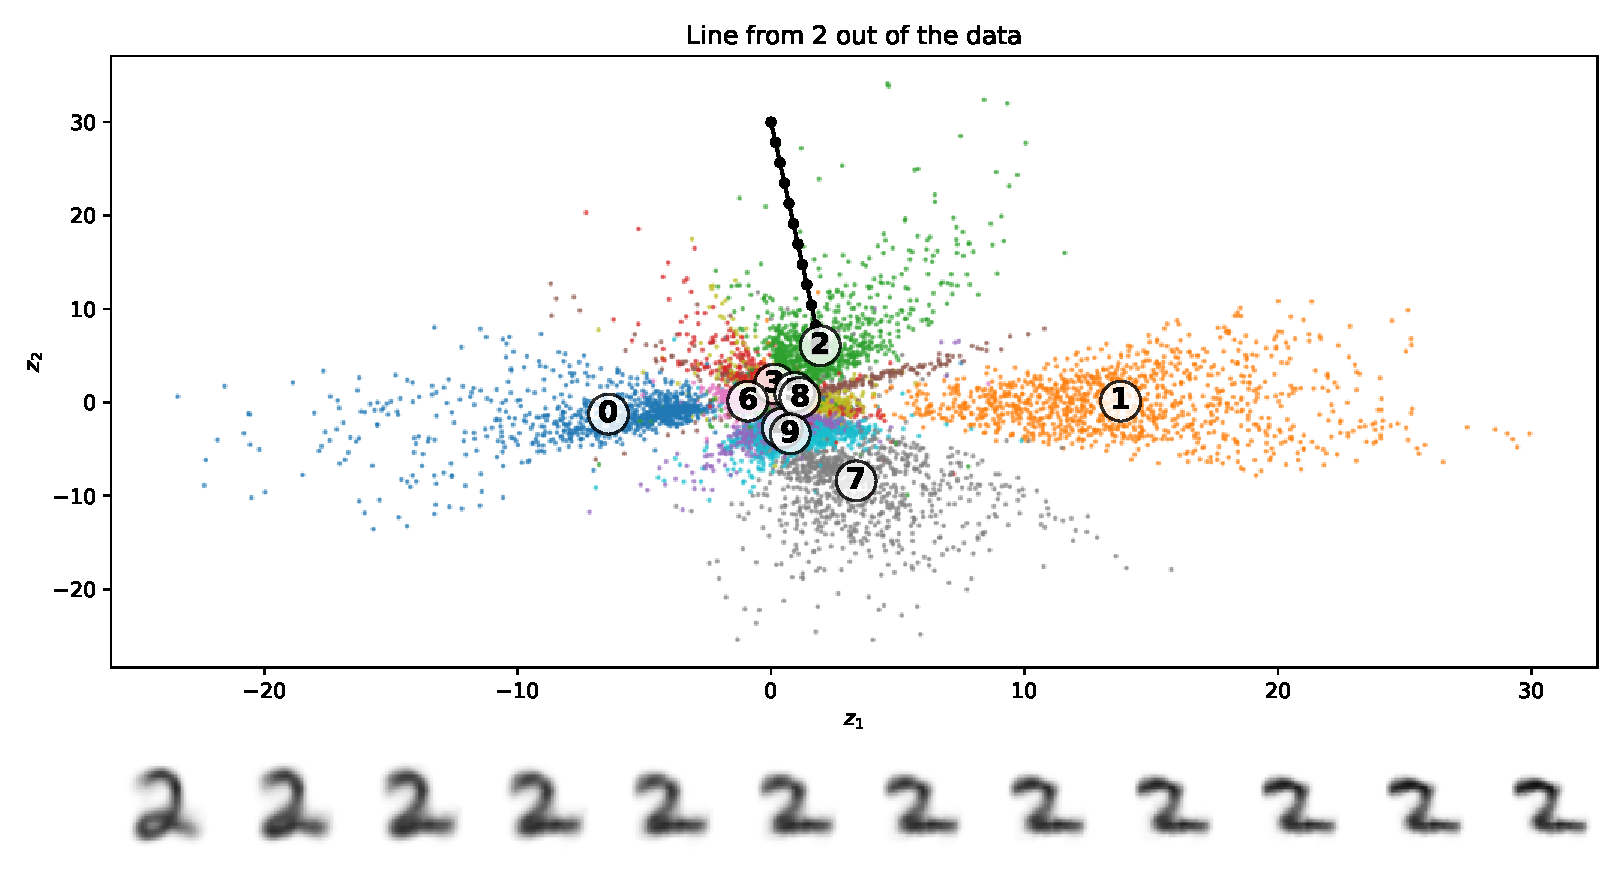
\includegraphics[width=\textwidth,height=0.82\textheight,keepaspectratio]{latent_line_out.pdf}
\end{center}
\end{frame}

\begin{frame}
  \frametitle{Decoding a grid over the latent space}
\begin{center}
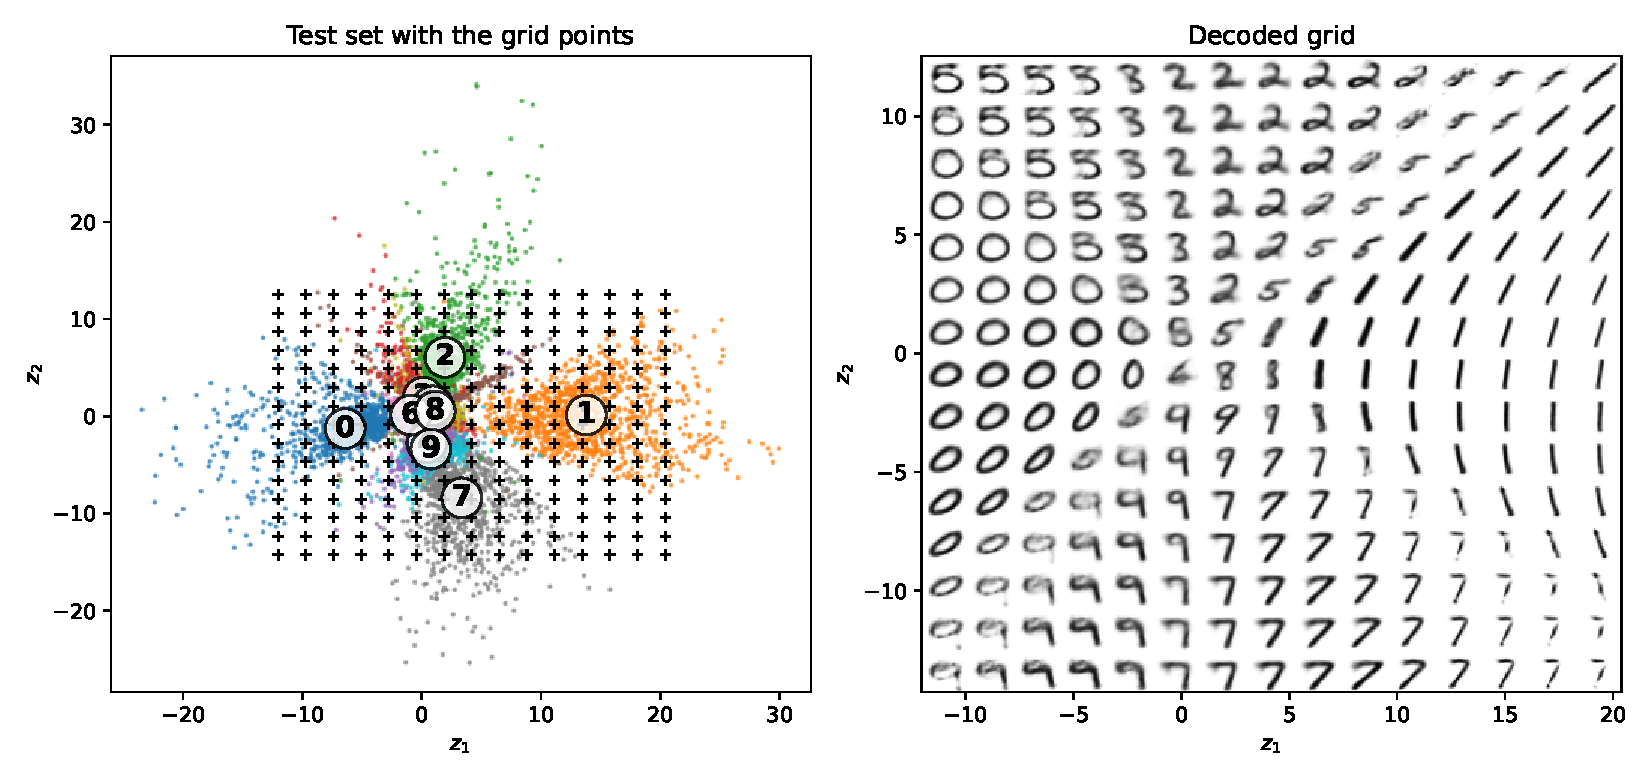
\includegraphics[width=\textwidth,height=0.82\textheight,keepaspectratio]{latent_grid.pdf}
\end{center}
\end{frame}

\begin{frame}
  \frametitle{So}
\vfill
\textbf{T}his gives a latent space, but not a generative model.
\vfill
\end{frame}


\begin{frame}
  \frametitle{Generative model}
\vfill
\begin{center}
\textbf{A} \textsl{generative model} is a probability distribution over the data that we can sample from, so it can produce new examples that look like the training data.
\end{center}
\vfill
\end{frame}

\begin{frame}
  \frametitle{The variational auto-encoder: the engineering idea}
\vfill
$$
\text{original} \rightarrow \text{latent} \rightarrow \textcolor{red}{\text{latent + noise}} \rightarrow \text{reconstruction}
$$
\vfill
\textbf{A}dding noise to the latent representation means nearby points must decode to similar images, so the gaps get filled in, `stitching together' the representation.
\vfill
\end{frame}

\begin{frame}
  \frametitle{The variational auto-encoder: the engineering idea}
\vfill
$$
\text{original} \rightarrow \text{latent} \rightarrow \textcolor{red}{\text{latent + noise}} \rightarrow \text{reconstruction}
$$
\vfill
\textbf{H}owever the network could cheat by spreading the latent points far apart so the noise doesn't matter; to stop this we also pull the latent points towards the origin.
\vfill
\end{frame}

\begin{frame}
  \frametitle{The variational auto-encoder: formally}
\vfill
$$
\mathbf{x} \rightarrow
\begin{array}{c}\boldsymbol{\mu}=f_\mu(\mathbf{x})\\ \boldsymbol{\sigma}=f_\sigma(\mathbf{x})\end{array}
\rightarrow
\textcolor{red}{z_i\sim\text{Normal}(\mu_i,\sigma_i)}
\rightarrow
\hat{\mathbf{x}}=g(\mathbf{z})
$$
\vfill
\textbf{T}he loss is
$$
L=\text{reconstruction error}+\sum_i\mathrm{KL}\big(\text{Normal}(\mu_i,\sigma_i)\,\|\,\text{Normal}(0,1)\big),
$$
where the KL term is what pulls the latent points towards the origin.
\vfill
\end{frame}

\begin{frame}
  \frametitle{Technical aside: the reparameterisation trick}
\vfill
We cannot backpropagate through a random sample, so instead we write
$$
z_i=\mu_i+\sigma_i\xi_i,\qquad \xi_i\sim\text{Normal}(0,1).
$$
\vfill
The randomness is now in $\xi_i$, which does not depend on the network, and $z_i$ is a differentiable function of $\mu_i$ and $\sigma_i$.
\vfill
\end{frame}

\begin{frame}
  \frametitle{The generative model}
\vfill
\textsl{T}hink of the decoder as a story about how a digit is made:
$$
\textcolor{red}{z_i\sim\text{Normal}(0,1)} \rightarrow x_j\sim\text{Bernoulli}\big(g_j(\mathbf{z})\big)
$$
where $j\in \{1,2,\ldots, 784\}$ labels pixels and $x_j$ is the pixel value.
\vfill
\begin{itemize}
\item \textbf{F}irst pick a point in latent space from a fixed, simple distribution, the \emph{prior} $p(\mathbf{z})$.
\item \textbf{T}hen the decoder gives a probability for each pixel being on, the \emph{likelihood} $p(\mathbf{x}|\mathbf{z})$.
\end{itemize}
\vfill
\end{frame}

\begin{frame}
  \frametitle{The generative model}
\vfill
\textsl{T}hink of the decoder as a story about how a digit is made:
$$
\textcolor{red}{z_i\sim\text{Normal}(0,1)} \rightarrow x_j\sim\text{Bernoulli}\big(g_j(\mathbf{z})\big)
$$
\vfill
It is like $\mathbf{z}$ is the idea and it has been `disguised' as an image. 
\vfill
\end{frame}


\begin{frame}
  \frametitle{The encoder}
\vfill
\textbf{G}iven a digit $\mathbf{x}$, which $\mathbf{z}$ produced it? That is the \textsl{posterior}.
$$
p(\mathbf{z}|\mathbf{x})=\frac{p(\mathbf{x}|\mathbf{z})\,p(\mathbf{z})}{p(\mathbf{x})},
$$
but $p(\mathbf{x})=\int p(\mathbf{x}|\mathbf{z})p(\mathbf{z})\,d\mathbf{z}$ is intractable.
\vfill
\textbf{S}o we approximate it:
$$
q(\mathbf{z}|\mathbf{x}):\quad z_i\sim\text{Normal}(\mu_i,\sigma_i),\qquad \boldsymbol{\mu}=f_\mu(\mathbf{x}),\ \boldsymbol{\sigma}=f_\sigma(\mathbf{x}).
$$
\textbf{T}he encoder is \emph{amortised} inference: one network gives the approximate posterior for every $\mathbf{x}$.
\vfill
\end{frame}

\begin{frame}
  \frametitle{The encoder}
\vfill
$$
q(\mathbf{z}|\mathbf{x}):\quad z_i\sim\text{Normal}(\mu_i,\sigma_i),\qquad \boldsymbol{\mu}=f_\mu(\mathbf{x}),\ \boldsymbol{\sigma}=f_\sigma(\mathbf{x}).
$$
\textbf{W}e are following the general deep learning philosophy, if there is some function we don't know we make a function for it. 
\vfill
\end{frame}

\begin{frame}
  \frametitle{Where the loss comes from}
\vfill
\textbf{W}e want to maximise $\log p(\mathbf{x})$ over the training data: this is maximum likelihood, and it fits the model's distribution to the data's.
\vfill
\end{frame}

\begin{frame}
  \frametitle{Where the loss comes from}
\vfill
\textbf{S}ince $p(\mathbf{x})=p(\mathbf{x},\mathbf{z})/p(\mathbf{z}|\mathbf{x})$ for any $\mathbf{z}$, we can average over $\mathbf{z}\sim q(\mathbf{z}|\mathbf{x})$ and multiply and divide by $q$:
$$
\log p(\mathbf{x})
=\mathbb{E}_q\left[\log\frac{p(\mathbf{x},\mathbf{z})}{q(\mathbf{z}|\mathbf{x})}\right]
+\mathbb{E}_q\left[\log\frac{q(\mathbf{z}|\mathbf{x})}{p(\mathbf{z}|\mathbf{x})}\right].
$$
\vfill
\end{frame}

\begin{frame}
  \frametitle{Where the loss comes from}
\vskip 0.25cm
\textbf{A} bit of algebra gives
$$
\log p(\mathbf{x})=\underbrace{\mathbb{E}_{q}\big[\log p(\mathbf{x}|\mathbf{z})\big]-\mathrm{KL}\big(q(\mathbf{z}|\mathbf{x})\,\|\,p(\mathbf{z})\big)}_{\text{ELBO (evidence lower bound)}}+\mathrm{KL}\big(q(\mathbf{z}|\mathbf{x})\,\|\,p(\mathbf{z}|\mathbf{x})\big).
$$
\begin{itemize}
\item \textbf{T}he last KL is non-negative, so the ELBO is a lower bound on $\log p(\mathbf{x})$, and maximising it improves both the model and the approximation $q$.
\item \textbf{T}he first term is minus the binary cross-entropy: the reconstruction error.
\item \textbf{T}he second is the KL to $\text{Normal}(0,1)$.
\end{itemize}
\vskip 0.25cm
\textbf{S}o the loss we guessed on engineering grounds is $L=-\text{ELBO}$.
\end{frame}


  \begin{frame}
    \frametitle{A VAE for MNIST}
  \vfill
  $$
  784 \rightarrow 512 \rightarrow 256 \rightarrow
  \begin{array}{c}\boldsymbol{\mu}\in\mathbb{R}^2\\ \log\boldsymbol{\sigma}^2\in\mathbb{R}^2\end{array}
  \rightarrow \mathbf{z}\in\mathbb{R}^2 \rightarrow 256 \rightarrow 512 \rightarrow 784
  $$
  \vfill
  Same layers as before; the encoder outputs $\log\boldsymbol{\sigma}^2$ rather than $\boldsymbol{\sigma}$ so it does not need to be kept positive.
  \vfill
  \end{frame}

\begin{frame}
  \frametitle{Auto-encoder and VAE latent spaces}
\vfill
\begin{center}
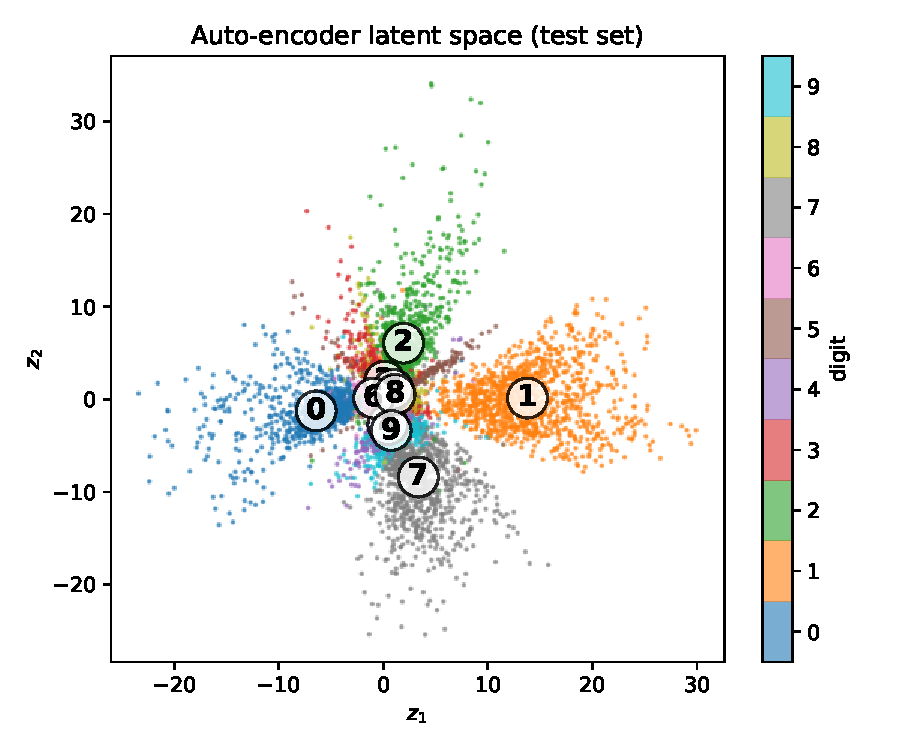
\includegraphics[width=0.49\textwidth,height=0.7\textheight,keepaspectratio]{latent_scatter.pdf}
\hfill
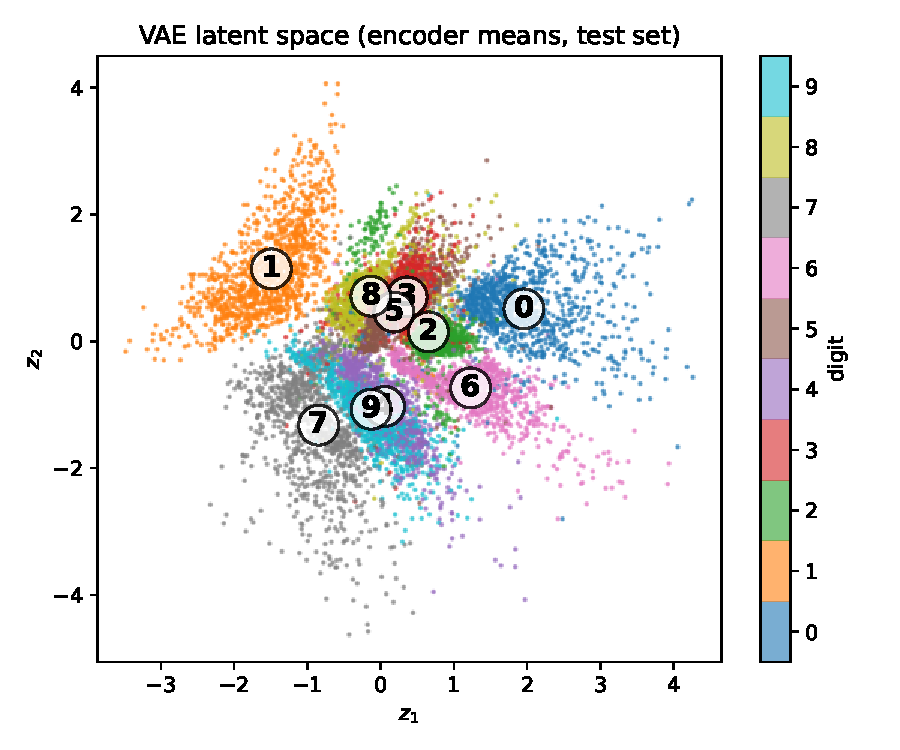
\includegraphics[width=0.49\textwidth,height=0.7\textheight,keepaspectratio]{vae_latent_scatter.pdf}
\end{center}
\vfill
The VAE latent space is compact, centred on the origin and has no gaps between the clusters.
\end{frame}

\begin{frame}
  \frametitle{VAE reconstructions}
\vfill
\begin{center}
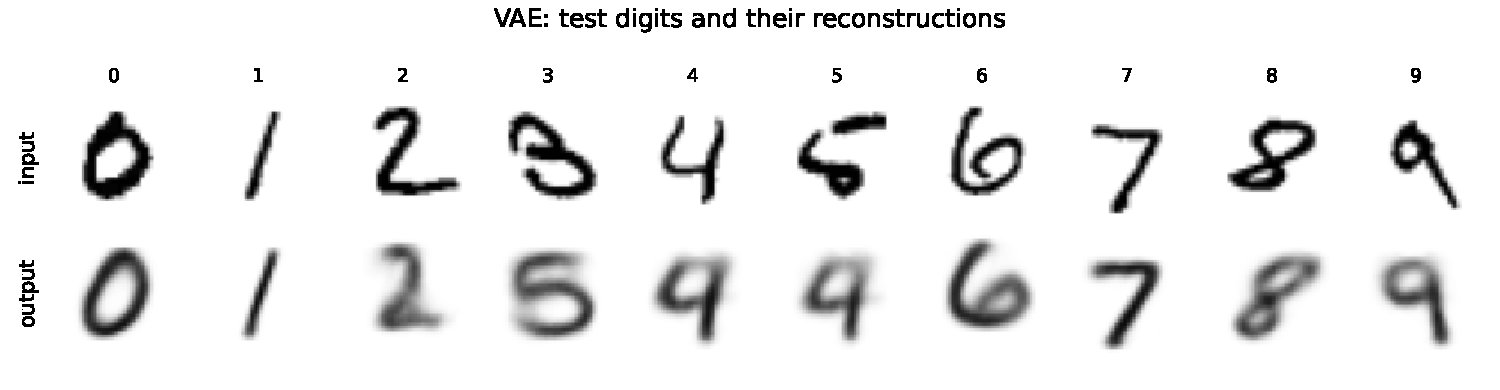
\includegraphics[width=\textwidth,height=0.7\textheight,keepaspectratio]{vae_reconstructions.pdf}
\end{center}
\vfill
A little blurrier than the auto-encoder: the price of the KL term.
\end{frame}

\begin{frame}
  \frametitle{VAE: a line from 0 to 2}
\begin{center}
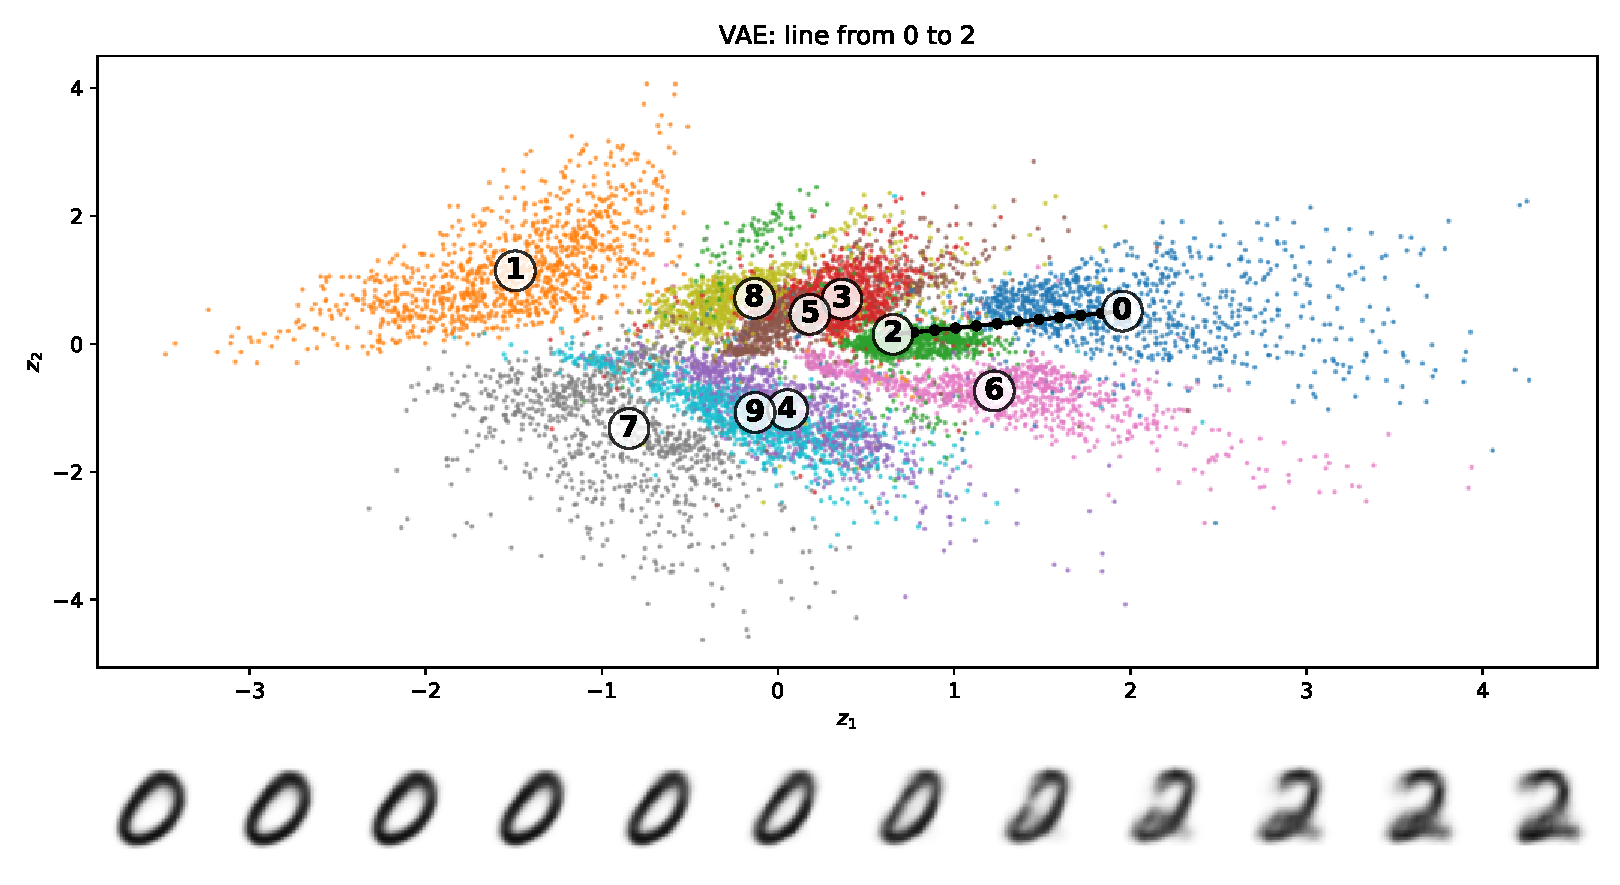
\includegraphics[width=\textwidth,height=0.72\textheight,keepaspectratio]{vae_latent_line_0_2.pdf}
\end{center}
Compare with the auto-encoder: the path between clusters now decodes to digits throughout.
\end{frame}

\begin{frame}
  \frametitle{VAE: a line from 1 to 0}
\begin{center}
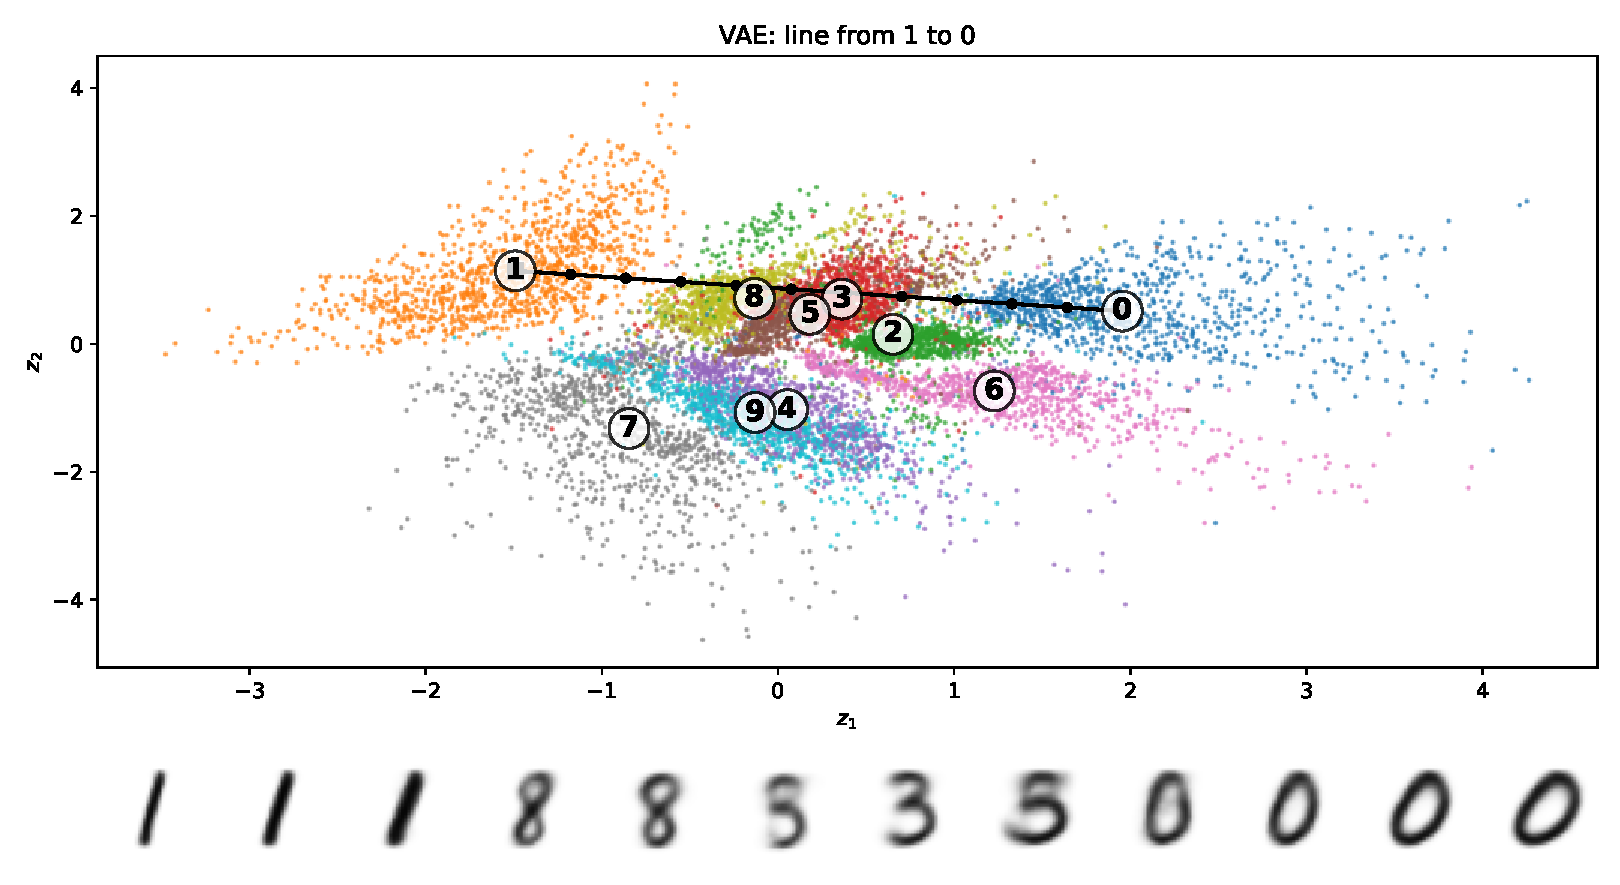
\includegraphics[width=\textwidth,height=0.82\textheight,keepaspectratio]{vae_latent_line_1_0.pdf}
\end{center}
\end{frame}

\begin{frame}
  \frametitle{VAE: a circle in latent space}
\begin{center}
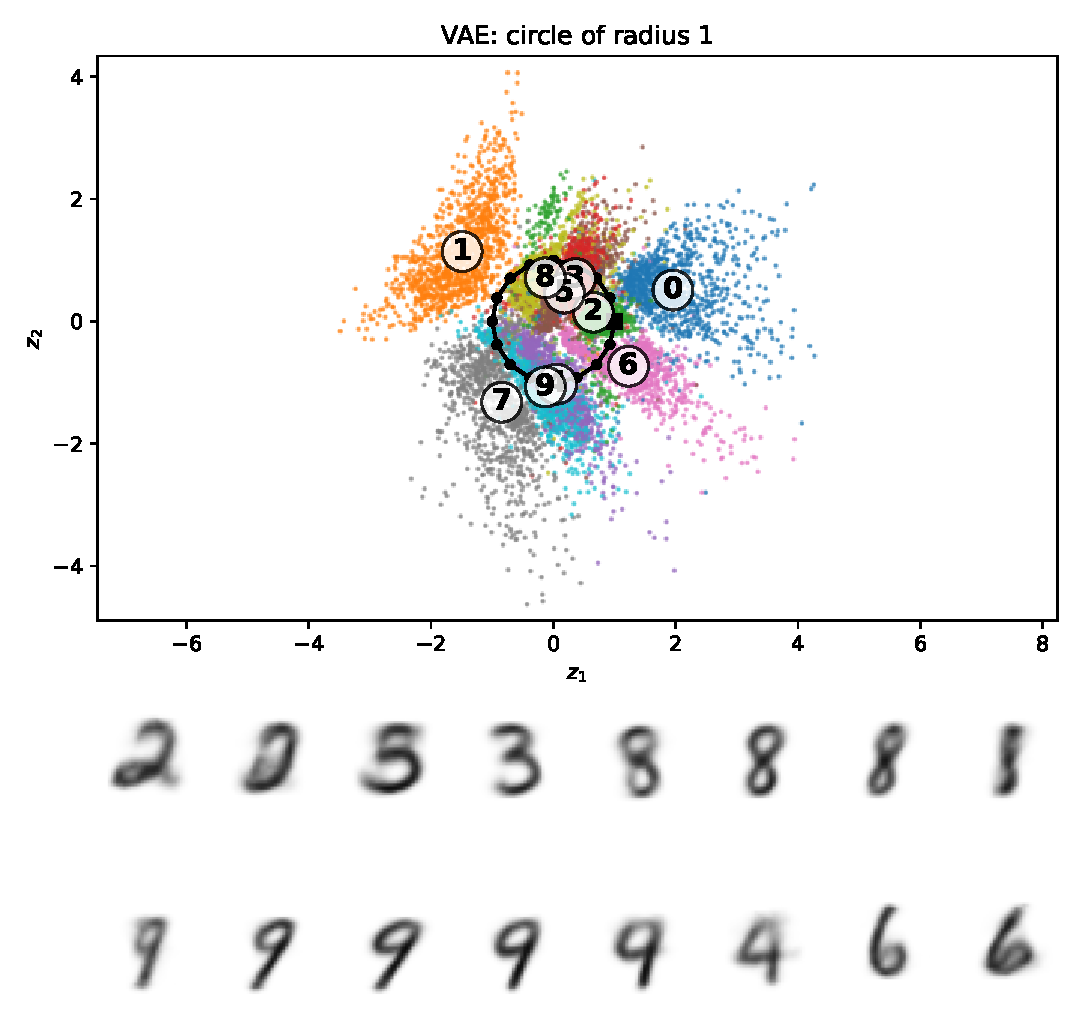
\includegraphics[width=\textwidth,height=0.82\textheight,keepaspectratio]{vae_latent_circle_1.pdf}
\end{center}
\end{frame}

\begin{frame}
  \frametitle{VAE: decoding a grid over the latent space}
\begin{center}
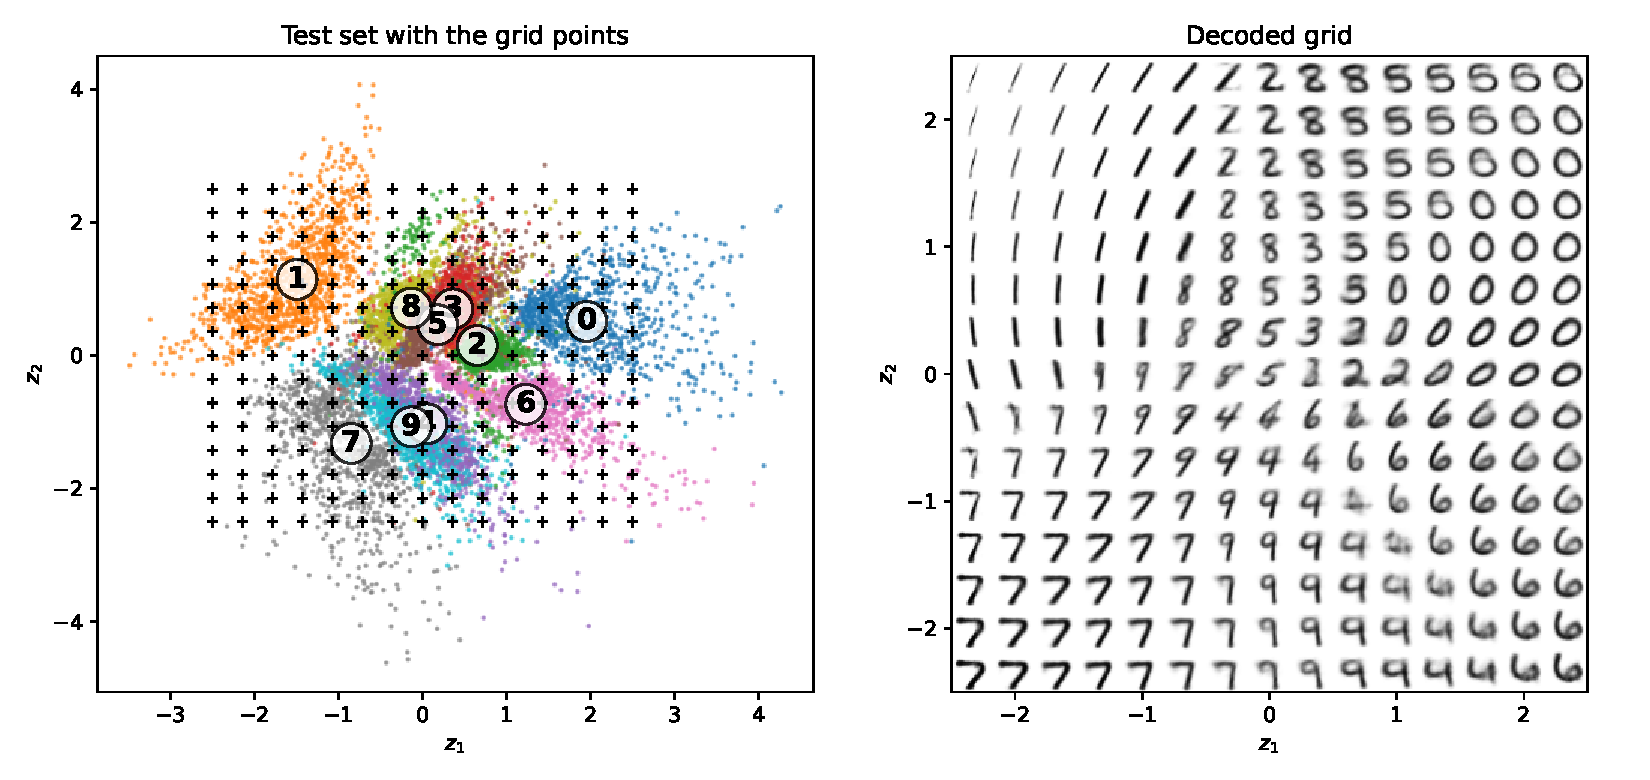
\includegraphics[width=\textwidth,height=0.82\textheight,keepaspectratio]{vae_latent_grid.pdf}
\end{center}
\end{frame}

\begin{frame}
  \frametitle{New digits}
\vfill
$$
\textcolor{red}{z_i\sim\text{Normal}(0,1)} \rightarrow \hat{\mathbf{x}}=g(\mathbf{z})
$$
\begin{center}
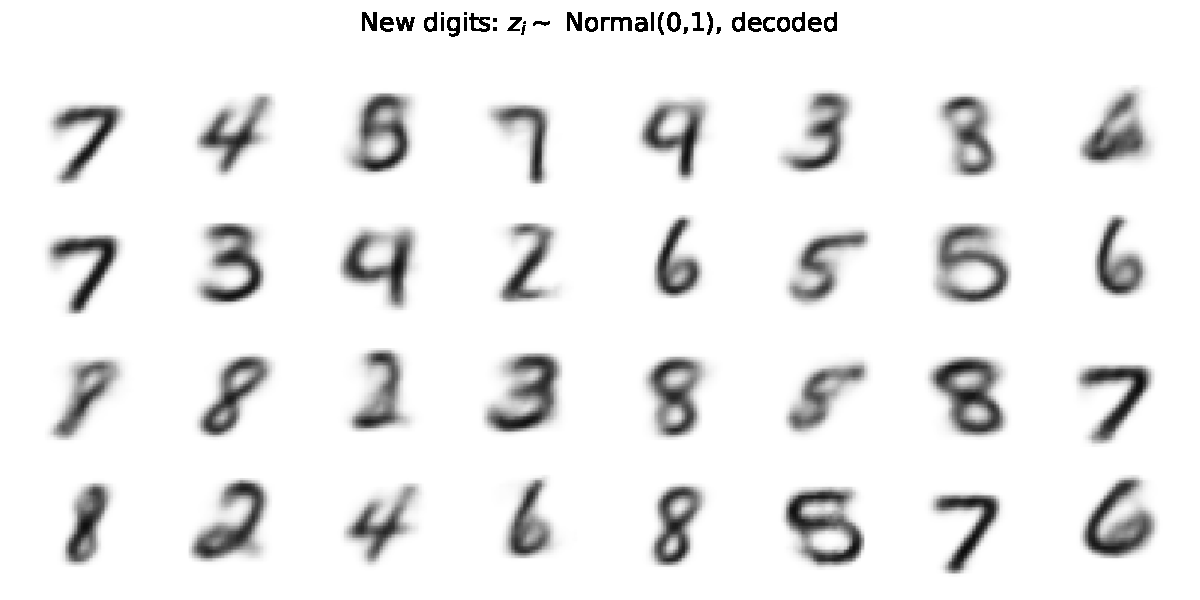
\includegraphics[width=\textwidth,height=0.6\textheight,keepaspectratio]{vae_samples.pdf}
\end{center}
\vfill
\end{frame}


\end{document}